%!TeX program = lualatex
\renewcommand{\thelektion}{L08 \textperiodcentered{} Logische Gatter I}
\usetikzlibrary{circuits.logic.US}
\graphicspath{{./Grundlagen_Info/16_ComputerUndKodierungen/Slides/assets}}

\begin{frame}\lessontitle{Lektion 08}{Logische Gatter I}{Vom Stromkreis zum Gatter: NOT, AND, OR \textperiodcentered{} Skript, Kapitel 4}\end{frame}

\begin{frame}\FDUtitle{Vom Stromkreis zur Information}
\begin{center}
Ein Chip ist ein Netzwerk aus leitenden Verbindungen und Schaltern.
\vspace{4mm}

\textbf{Zentrale Idee}: Elektrische Zustände werden als logische Zustände interpretiert.
\end{center}
\begin{figure}[H]
    \centering
    \begin{tikzpicture}[scale=1.0]
    \begin{scope}[shift={(0,0)}, local bounding box=openBB]
        \coordinate (open-base) at (0,0);
        \coordinate (open-bat-bot) at ($(open-base)+(0.6,0.8)$);
        \coordinate (open-bat-top) at ($(open-base)+(0.6,2.2)$);
        \coordinate (open-sw-left) at ($(open-base)+(2.0,2.2)$);
        \coordinate (open-sw-right) at ($(open-base)+(2.9,2.2)$);
        \coordinate (open-lamp) at ($(open-base)+(3.8,2.2)$);
        \coordinate (open-ret) at ($(open-base)+(3.8,0.8)$);

        \draw (open-bat-bot) -- (open-bat-top);
        \draw ($(open-base)+(0.45,1.15)$) -- ($(open-base)+(0.75,1.15)$);
        \draw ($(open-base)+(0.50,1.60)$) -- ($(open-base)+(0.70,1.60)$);
        \node[left] at ($(open-base)+(0.35,1.35)$) {$U$};

        \draw (open-bat-top) -- (open-sw-left);
        \draw (open-sw-left) -- ($(open-sw-left)+(0.6,0.3)$);
        \draw (open-sw-right) -- (open-lamp);
        \draw (open-lamp) circle (0.35);
        \draw ($(open-base)+(3.55,1.95)$) -- ($(open-base)+(4.05,2.45)$);
        \draw (open-bat-bot) -- (open-ret) -- ($(open-lamp)+(0,-0.35)$);

        \node at ($(open-base)+(2.35,2.65)$) {\tiny kein Kontakt};
        \node at ($(open-base)+(3.8,1.3)$) {Last aus};
        \node at ($(open-base)+(2.5,2.95)$) {Schalter offen};
    \end{scope}
    \node[draw,rounded corners,fit=(openBB),inner sep=8pt] {};

    \begin{scope}[shift={(6.2,0)}, local bounding box=closedBB]
        \coordinate (closed-base) at (0,0);
        \coordinate (closed-bat-bot) at ($(closed-base)+(0.6,0.8)$);
        \coordinate (closed-bat-top) at ($(closed-base)+(0.6,2.2)$);
        \coordinate (closed-sw-left) at ($(closed-base)+(2.0,2.2)$);
        \coordinate (closed-sw-right) at ($(closed-base)+(2.6,2.2)$);
        \coordinate (closed-lamp) at ($(closed-base)+(3.8,2.2)$);
        \coordinate (closed-ret) at ($(closed-base)+(3.8,0.8)$);

        \draw (closed-bat-bot) -- (closed-bat-top);
        \draw ($(closed-base)+(0.45,1.15)$) -- ($(closed-base)+(0.75,1.15)$);
        \draw ($(closed-base)+(0.50,1.60)$) -- ($(closed-base)+(0.70,1.60)$);
        \node[left] at ($(closed-base)+(0.35,1.35)$) {$U$};

        \draw (closed-bat-top) -- (closed-sw-left);
        \fill (closed-sw-left) circle (0.04);
        \fill (closed-sw-right) circle (0.04);
        \draw[line width=0.5pt] (closed-sw-left) -- (closed-sw-right);
        \draw (closed-sw-right) -- (closed-lamp);
        \draw (closed-lamp) circle (0.35);
        \fill (closed-lamp) circle (0.12);
        \draw (closed-bat-bot) -- (closed-ret) -- ($(closed-lamp)+(0,-0.35)$);

        \node at ($(closed-base)+(2.3,2.65)$) {\tiny Kontakt};
        \node at ($(closed-base)+(3.8,1.3)$) {Last aktiv};
        \node at ($(closed-base)+(2.5,2.95)$) {Schalter geschlossen};
    \end{scope}
    \node[draw,rounded corners,fit=(closedBB),inner sep=8pt] {};
\end{tikzpicture}

    \[
    \text{niedrige Spannung} \longleftrightarrow 0
    \qquad
    \qquad
    \text{hohe Spannung} \longleftrightarrow 1
\]
\end{figure}
\end{frame}

\begin{frame}\FDUtitle{Warum ausgerechnet zwei Zustände?}
\begin{itemize}[<+->]\setlength\itemsep{7pt}
  \item In echten Schaltungen gibt es Rauschen, Verzögerungen, Fertigungstoleranzen
  \item Man arbeitet daher mit \tib{Spannungsbereichen}, nicht mit exakten Werten
  \item Zwei klar unterscheidbare Zustände lassen sich sehr zuverlässig erkennen
\end{itemize}
\vspace{3mm}
\begin{center}
Erinnerung an Lektion 1: Shannon zeigte 1937, dass sich Boolesche Logik so elektrisch realisieren lässt.
\end{center}
\end{frame}

\begin{frame}\FDUtitle{Vom Transistor zum Gatter}
\begin{itemize}[<+->]\setlength\itemsep{7pt}
  \item \tib{Transistoren} = extrem schnelle elektronische Schalter
  \item Ein logisches \tib{Gatter} ist eine konkrete Schaltung aus mehreren Transistoren
  \item Reale Gatter haben technische Kennwerte: Propagationsverzögerung, Leistungsaufnahme, Fan-out
\end{itemize}
\end{frame}

\begin{frame}\FDUtitle{Boolesche Grundverknüpfungen}
\begin{center}
Funktionen, die Bits als Eingabe erhalten und \textbf{genau ein} Bit ausgeben.
\end{center}
\vspace{4mm}
\begin{center}
\Large\bfseries\color{FDUteal}NOT \quad AND \quad OR
\end{center}
\end{frame}

\begin{frame}\FDUtitle{NOT -- Negation}
\begin{columns}[c,onlytextwidth]
\begin{column}{.46\textwidth}
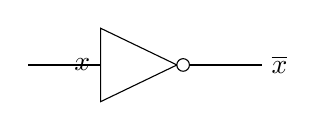
\begin{tikzpicture}[circuit logic US, scale=1.3]
    \node[not gate, draw] (not1) {};
    \draw (not1.input) ++(-0.7,0) -- (not1.input) node[left] {$x$};
    \draw (not1.output) -- ++(0.7,0) node[right] {$\overline{x}$};
\end{tikzpicture}

\end{column}
\begin{column}{.46\textwidth}
\begin{tabular}{cc}
    $x$ & $\overline{x}$ \\\midrule
    0 & 1 \\
    1 & 0 \\
\end{tabular}
\end{column}
\end{columns}
\vspace{3mm}
\begin{center}Ein Eingang, negierter Ausgang.\end{center}
\end{frame}

\begin{frame}\FDUtitle{AND -- Konjunktion}
\begin{columns}[c,onlytextwidth]
\begin{column}{.46\textwidth}
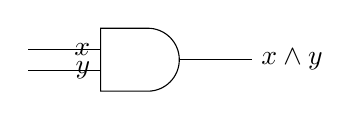
\begin{tikzpicture}[circuit logic US, scale=1.3]
    \node[and gate, draw] (and1) {};
    \draw (and1.input 1) ++(-0.7,0) -- (and1.input 1) node[left] {$x$};
    \draw (and1.input 2) ++(-0.7,0) -- (and1.input 2) node[left] {$y$};
    \draw (and1.output) -- ++(0.7,0) node[right] {$x \wedge y$};
\end{tikzpicture}

\end{column}
\begin{column}{.46\textwidth}
\begin{tabular}{ccc}
    $x$ & $y$ & $x \wedge y$ \\\midrule
    0 & 0 & 0 \\
    0 & 1 & 0 \\
    1 & 0 & 0 \\
    1 & 1 & 1 \\
\end{tabular}
\end{column}
\end{columns}
\vspace{3mm}
\begin{center}Ausgang 1 nur, wenn \textbf{beide} Eingänge 1 sind.\end{center}
\end{frame}

\begin{frame}\FDUtitle{OR -- Disjunktion}
\begin{columns}[c,onlytextwidth]
\begin{column}{.46\textwidth}
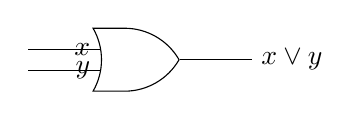
\begin{tikzpicture}[circuit logic US, scale=1.3]
    \node[or gate, draw] (or1) {};
    \draw (or1.input 1) ++(-0.7,0) -- (or1.input 1) node[left] {$x$};
    \draw (or1.input 2) ++(-0.7,0) -- (or1.input 2) node[left] {$y$};
    \draw (or1.output) -- ++(0.7,0) node[right] {$x \vee y$};
\end{tikzpicture}

\end{column}
\begin{column}{.46\textwidth}
\begin{tabular}{ccc}
    $x$ & $y$ & $x \vee y$ \\\midrule
    0 & 0 & 0 \\
    0 & 1 & 1 \\
    1 & 0 & 1 \\
    1 & 1 & 1 \\
\end{tabular}
\end{column}
\end{columns}
\vspace{3mm}
\begin{center}Ausgang 1, wenn \textbf{mindestens ein} Eingang 1 ist.\end{center}
\end{frame}

\begin{frame}{Auftrag}{Kapitel 4: Logische Grundverknüpfungen}
\aufgabebox{\textbf{Aufgabe 4.3}}
\begin{center}
Ein Fahrstuhl darf sich nur bewegen, wenn die Tür geschlossen \emph{und} entweder das zulässige Gewicht nicht überschritten \emph{oder} der Notfall-Modus aktiviert ist.
\vspace{4mm}

Modellieren Sie diese Bedingung mit AND-, OR- und NOT-Gattern grafisch und geben Sie die zugehörige logische Formel an.
\end{center}
\end{frame}

\begin{frame}\FDUtitle{Lösung: Aufgabe 4.3}
\begin{center}
Ein Fahrstuhl darf sich nur bewegen, wenn die Tür geschlossen \emph{und} entweder das zulässige Gewicht nicht überschritten \emph{oder} der Notfall-Modus aktiviert ist.
\end{center}
\begin{center}
Mit $t=$ \enquote{Tür geschlossen}, $u=$ \enquote{Zulässiges Gewicht überschritten}, $n=$ \enquote{Notfall-Modus aktiv} lautet die Formel:
\large $t \wedge (\overline{u} \vee n)$\end{center}
    \centering
    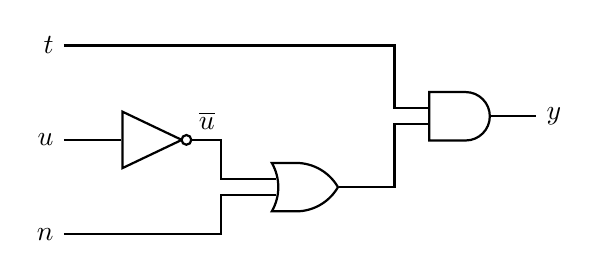
\begin{tikzpicture}[circuit logic US, thick]
    \node[not gate, draw] (not-u) at (1,0.6) {};
    \node[or gate, draw] (or1) at (3,0) {};
    \node[and gate, draw] (and1) at (5,0.9) {};

    \draw (0,0.6) node[left] {$u$} -- (not-u.input);
    \draw (not-u.output) -- (2,0.6) node[midway, above] {$\overline{u}$}
        |- (or1.input 1);
    \draw (0,-0.6) node[left] {$n$} -- (2,-0.6)
        |- (or1.input 2);

    % Das Türsignal umgeht die Negation und wird erst am AND-Gatter verknüpft.
    \draw (0,1.8) node[left] {$t$} -- (4.2,1.8) |- (and1.input 1);
    \draw (or1.output) -- (4.2,0) |- (and1.input 2);
    \draw (and1.output) -- (6,0.9) node[right] {$y$};
\end{tikzpicture}

\end{frame}
